\documentclass[aspectratio=169,11pt]{beamer}
\makeatletter
\input{../../templates/dune-professional/beamerthemeDUNEProfessional.sty}
\makeatother
\DuneUseWhite
% Meeting branding is local to this deck; the shared white profile is unchanged.
\newcommand{\DpsMeetingDate}{November 2026}
\newcommand{\mydate}{\DpsMeetingDate}
\newcommand{\DpsFermilabLogo}{%
  \includegraphics[height=2.8mm]{\DuneLogoPath/FNAL-Logo-Black.pdf}%
}
\setbeamertemplate{footline}{%
  \leavevmode%
  \begin{beamercolorbox}[wd=\paperwidth,ht=6.5mm,dp=0mm]{footline}%
    \begin{tikzpicture}[remember picture,overlay]
      \node[anchor=west,inner sep=0pt]
        at ([xshift=0.78cm,yshift=3.2mm]current page.south west) {\DpsFermilabLogo};
      \node[text=DuneTextMuted,font=\footnotesize,inner sep=0pt]
        at ([yshift=3.2mm]current page.south)
        {I\&I meeting\enspace|\enspace\DpsMeetingDate};
      \node[anchor=east,text=DuneTextMuted,font=\footnotesize,inner sep=0pt]
        at ([xshift=-0.78cm,yshift=3.2mm]current page.south east) {\insertframenumber};
    \end{tikzpicture}%
  \end{beamercolorbox}%
}

% Large grey DUNE branding on the title and transitions, without any footer.
\setbeamertemplate{title page}{%
  \begin{tikzpicture}[remember picture,overlay]
    \node[inner sep=0pt]
      at ([xshift=-4cm]current page.center)
      {\includegraphics[width=5.2cm,trim=2bp 2bp 2bp 2bp,clip]{\DuneLogoPath/DUNElogo_gray.pdf}};
    \node[text=DuneText,font=\bfseries\fontsize{23}{28}\selectfont,
      anchor=west,align=flush left,text width=7.2cm,inner sep=0pt]
      at ([xshift=7.2cm,yshift=-3.1cm]current page.north west) {\inserttitle};
    \node[text=DuneTextMuted,font=\large,anchor=west,align=left,text width=8cm,inner sep=0pt]
      at ([xshift=7.2cm,yshift=-4.65cm]current page.north west) {\insertsubtitle};
    \node[text=DuneText,font=\large\bfseries,anchor=west,inner sep=0pt]
      at ([xshift=7.2cm,yshift=-6.5cm]current page.north west) {\insertauthor};
    \node[text=DuneTextMuted,font=\normalsize,anchor=west,inner sep=0pt]
      at ([xshift=7.2cm,yshift=-7.15cm]current page.north west) {\insertdate};
  \end{tikzpicture}%
}

\newcommand{\DpsSectionTransition}[1]{%
  \begin{frame}[plain]
    \begin{tikzpicture}[remember picture,overlay]
      \node[inner sep=0pt]
        at ([xshift=-4cm]current page.center)
        {\includegraphics[width=5.2cm,trim=2bp 2bp 2bp 2bp,clip]{\DuneLogoPath/DUNElogo_gray.pdf}};
      \node[text=DuneText,font=\bfseries\fontsize{30}{36}\selectfont,inner sep=0pt]
        at ([xshift=2cm]current page.center) {#1};
    \end{tikzpicture}
  \end{frame}%
}
\newcommand{\DpsDetectorTransition}{\DpsSectionTransition{Detector}}
\newcommand{\DpsBackupsTransition}{\DpsSectionTransition{Backups}}

\title{VD Detector Protection System}
\subtitle{Status and work towards a \\ DPS conceptual design}
\author{Manuel Arroyave}
\date{I\&I meeting --- \DpsMeetingDate}
\hypersetup{colorlinks=true,urlcolor=DuneInfo,linkcolor=DuneInfo}
\newcommand{\captionline}[1]{\par{\footnotesize\color{DuneTextMuted}#1\par}}
% Schematic service boundary, not a surveyed section or controller inventory.
\newcommand{\siteboundarymap}{%
\begin{tikzpicture}[
 box/.style={draw=DuneTextMuted,fill=none,text=DuneText,align=center,font=\small,inner sep=4pt},
 level/.style={anchor=east,font=\small,text=DuneTextMuted}]
 \node[font=\small\bfseries,align=center,text width=2.0cm] at (1.25,2.25) {SDSTA\\site services};
 \node[font=\small\bfseries,align=center,text width=2.8cm] at (4.05,2.25) {FFDG DUNE FD\\building services};
 \node[level] at (-0.05,1.25) {Surface};
 \node[box,text width=1.95cm] (surface) at (1.25,1.25) {Oro Hondo\\Ross shaft};
 \node[level] at (-0.05,0.25) {4850};
 \node[box,text width=2.8cm] at (4.05,0.25) {CUC / caverns\\HVAC, chilled water};
 \node[level] at (-0.05,-0.85) {4910};
 \node[box,text width=2.8cm] at (4.05,-0.85) {SP-1 / SP-2\\sump interfaces};
 \node[box,text width=1.95cm] (drainage) at (1.25,-1.85) {Mine drainage\\and pumping};
 \draw[draw=DuneTextMuted,line width=0.7pt] (surface.south) -- (drainage.north);
 \draw[-{Stealth},draw=DuneTextMuted,line width=0.7pt] (3.1,-1.3) -- (2.35,-1.65);
\end{tikzpicture}%
}

% White-profile system diagrams: dark outlines, labels and explicit line meaning.
% Keep the same geometry as the native TikZ version of the October deck.
\tikzset{
  dps node/.style={
    dune repo muted,draw=DuneTextMuted,fill=none,text=DuneText,line width=0.7pt,
    rounded corners=0pt,font=\small,text width=2.8cm,
    minimum height=0.95cm,inner sep=5pt
  },
  dps controller/.style={dps node},
  dps load/.style={dps node},
  dps flow/.style={
    dune flow,-{Stealth[length=1.7mm,width=1.3mm]},
    draw=DuneTextMuted,line width=1pt
  },
  dps both/.style={
    dps flow,arrows={Stealth[length=1.7mm,width=1.3mm]-Stealth[length=1.7mm,width=1.3mm]}
  },
  dps power/.style={dps flow,draw=DuneText},
  dps label/.style={
    dune label,fill=none,text=DuneText,font=\small,inner sep=2pt
  },
  dps boundary/.style={draw=DuneTextMuted,fill=none,line width=0.7pt},
  dps heading/.style={text=DuneText,font=\small\bfseries,inner sep=0pt}
}

% The normal deck build compiles these sources; no external renderer is needed.
\newcommand{\dpsdiagram}[1]{%
  \begin{adjustbox}{max width=\linewidth,max totalheight=4.6cm}%
    \input{diagrams/#1.tikz.tex}%
  \end{adjustbox}%
}

% New meeting material. Keep all earlier slides and technical backups.
\newcommand{\DpsKnownAndMissing}{%
\begin{frame}{The hardware connection list is still growing}
\begin{columns}[T,onlytextwidth]
\begin{column}{0.47\textwidth}
\textbf{Known starting points}\par\medskip
Rack power distribution units (PDUs).\par\medskip
The TPC electronics / Bottom Drift Electronics (BDE) protection design and its test work.
\end{column}
\begin{column}{0.49\textwidth}
\textbf{Work still needed}\par\medskip
A complete list of hardware inputs, outputs and feedback between the equipment and the \\ DPS Programable Logic Controller.\par\medskip
A conceptual design covering all VD DPS connections.
\end{column}
\end{columns}\par\bigskip
\textbf{Approach:} extend the existing TPC/BDE protection schema based on a central PLC.\par\medskip
Target: gather the consortia and LBNF connection information by late January 2027.
\end{frame}%
}

\newcommand{\DpsFireScope}{%
\begin{frame}{Fire systems stay separate from detector protection}
\begin{columns}[T,onlytextwidth]
\begin{column}{0.47\textwidth}
\textbf{DPS scope}\par\medskip
Equipment protection: permits, inhibits, power state and confirmation of the response.
\end{column}
\begin{column}{0.49\textwidth}
\textbf{Separate fire-system scope}\par\medskip
Fire detection, fire alarms and emergency response remain outside DPS control.
\end{column}
\end{columns}\par\bigskip
\textbf{Could equipment status help responders?}\par\medskip
Possible feedback includes affected racks, power state, completed shutdowns and event times.\par\medskip
Ask the emergency response team which information would help. The need, route and responsibility for a feed are not agreed.\par\medskip
\captionline{Rack smoke-contact hardware remains in the reference material; it does not define a DPS fire-alarm system.}
\end{frame}%
}

\newcommand{\DpsFfdgUpdate}{%
\begin{frame}{How FFDG BSI status can support detector protection}
\renewcommand{\arraystretch}{1.25}
\begin{tabularx}{\textwidth}{@{}>{\RaggedRight\arraybackslash}p{4.2cm}>{\RaggedRight\arraybackslash}X@{}}
\toprule
\textbf{Reported in discussion} & \textbf{What we need to resolve}\\\midrule
No 24-hour support; issues attended next business day & Decide a schema of human informed decisions using this and what happens when it is unavailable.\\
Dedicated sensors recommended for critical equipment protection & Identify where detector-owned sensors are needed.\\
%Possible existing SDSTA exchange, including fire variables & Confirm the existing route and whether anyone needs additional information from DPS.\\
\bottomrule
\end{tabularx}\par\medskip
\textbf{BMS access alone does not establish a protection interface.}\par\medskip
%\captionline{From Manuel's commissioning update. Service commitments and interface suitability still need agreement.}
\end{frame}%
}

\newcommand{\DpsSdstaUpdate}{%
\begin{frame}{SDSTA proposes a restricted SCADA status interface}
\renewcommand{\arraystretch}{1.25}
\begin{tabularx}{\textwidth}{@{}>{\RaggedRight\arraybackslash}p{2.6cm}>{\RaggedRight\arraybackslash}X@{}}
\toprule
\textbf{Topic} & \textbf{Reported proposal / next input}\\\midrule
%System & SDSTA SCADA; a transition away from legacy Johnson systems was reported.\\
Interface & Modbus TCP, exposing a set of variables on selected ports. SDSTA retains control of its systems.\\
Write access & Status-only intent. Agree and check that the interface rejects writes and commands.\\
Variables & A list is pending, including Oro Hondo status and driver variables + HVAC.\\
\bottomrule
\end{tabularx}\par\medskip
\textbf{Still to agree:} variable meaning, data quality, loss-of-data behaviour and network access.\par\medskip
%\captionline{The protocol and platform transition are reported working inputs. They do not establish an installed or accepted interface.}
\end{frame}%
}

\newcommand{\DpsConnectionCollection}{%
\begin{frame}{Each group must identify its hardware connections}
\renewcommand{\arraystretch}{1.2}
\begin{tabularx}{\textwidth}{@{}>{\RaggedRight\arraybackslash}p{3.4cm}>{\RaggedRight\arraybackslash}X@{}}
\toprule
\textbf{For every connection} & \textbf{Record}\\\midrule
Source and destination & Equipment, rack / panel, connector, channel and drawing revision\\
Signal and interface & Measurement or state; units, normal / fault values; wired I/O or network protocol\\
Protection action & Condition, affected load, permit / inhibit and allowed response time\\
Feedback and recovery & Equipment response; lost-signal behaviour; reset and re-enable\\
Responsibility and gaps & Consortium or LBNF contact; evidence, missing items and next action\\
\bottomrule
\end{tabularx}\par\bigskip
Use one common register for the consortia and the LBNF facility. Each group confirms that its list covers its hardware.
\end{frame}%
}

\newcommand{\DpsExtendBde}{%
\begin{frame}{Extend the BDE approach into a full DPS concept}
\centering
\begin{tikzpicture}[
  box/.style={dps node,text width=2.7cm,minimum height=1.15cm},
  flow/.style={dps flow}]
  \node[box] (input) at (-5.1,0) {Hardware inputs\\and feedback};
  \node[box] (brain) at (-1.7,0) {DPS brain\\BDE-based PLC};
  \node[box] (output) at (1.7,0) {Remote I/O / PDUs\\Permits and inhibits};
  \node[box] (load) at (5.1,0) {Protected loads\\Response checks};
  \draw[flow] (input) -- (brain);
  \draw[flow] (brain) -- (output);
  \draw[flow] (output) -- (load);
\end{tikzpicture}\par\medskip
\raggedright\DuneDiagramCaption{Proposed extension of the existing TPC/BDE protection approach. Controller and I/O sizing follow the complete connection list.}\par\bigskip
Reuse the PLC, remote-I/O and protection-rule approach where it fits. Map the additional subsystem and facility interfaces.\par\medskip
SC carries operating requests and records equipment states and trips.\par\medskip
Test each added path from the fault input to confirmed equipment response.
\end{frame}%
}

\newcommand{\DpsMilestones}{%
\begin{frame}{Gather inputs by January; complete the design by April}
\begin{columns}[T,onlytextwidth]
\begin{column}{0.48\textwidth}
{\large\textbf{Late January 2027}}\par\medskip
\textbf{Gather the information}\par\medskip
Consortia and LBNF return their connections, limits and required actions.\par\medskip
Include feedback, response times and lost-signal behaviour.\par\medskip
Confirm coverage; name contacts and remaining gaps.
\end{column}
\begin{column}{0.48\textwidth}
{\large\textbf{Mid-April 2027}}\par\medskip
\textbf{Complete a comprehensive DPS design}\par\medskip
Architecture, controller and I/O allocation; interfaces and protection rules.\par\medskip
Fault response, shutdown order and recovery.\par\medskip
Drawings, parts, power needs and test plan; record open choices for review.
\end{column}
\end{columns}\par\bigskip
\textbf{Work in parallel:} use the Batavia and SURF benches to check representative protection paths as the design develops.
\captionline{Planning targets. Hardware qualification and installation are separate steps.}
\end{frame}%
}

\hyphenpenalty=10000
\exhyphenpenalty=10000
\begin{document}
\begin{frame}[plain]
  \titlepage
\end{frame}

\DpsKnownAndMissing

\begin{frame}{DPS protects equipment; SC operates and records}
\renewcommand{\arraystretch}{1.18}
\begin{tabularx}{\textwidth}{@{}>{\RaggedRight\arraybackslash}p{2.2cm}>{\RaggedRight\arraybackslash}X@{}}
\textbf{DPS} & Detector Protection System: arbitrates protection, applies permits and inhibits, and checks the response.\\
    \textbf{DSCS} & DUNE Detector Slow Controls System (SC): operates and monitors equipment, coordinates requests and keeps the logs.\\
\textbf{DAQ} & Data acquisition: configures readout and records detector data.\\
\textbf{BMS / Cryo / SCADA} & Building management, SCADA Controls and Cryogenics: operate their systems and report their state to SC.\\
\textbf{Consortia} & Define operating limits, protection actions and allowed response times.\\
\textbf{Local\newline interlocks} & Can trip equipment without SC or the central DPS.\\
\end{tabularx}\par\bigskip
\textbf{Protection trips take priority over operating requests.}\par\medskip
SDSTA issues personnel-safety alarms.
\end{frame}

%\DpsFireScope

\begin{frame}{Facility interfaces may connect to SC or the DPS PLC}
\centering
\dpsdiagram{overview}\par\smallskip
\raggedright\DuneDiagramCaption{Dashed: facility links under study. Cryogenics exchanges information in both directions.}\par\smallskip
\raggedright

The receiving endpoint may be SC/Ignition, the DPS PLC, or both; it is still to be agreed.\par\smallskip
SC $\leftrightarrow$ DPS: OPC UA. DPS $\leftrightarrow$ equipment: SNMP / EtherCAT.
\end{frame}

\begin{frame}{Build the DPS brain on the BDE PLC architecture}
\begin{itemize}
\item Industrial off-the-shelf hardware; modular I/O supports expansion and scaling.
\item Vendor support for maintenance and upgrades.
\item Reuse the BDE panels across the $\sim$70\,m mezzanine; extend to other systems.
\end{itemize}\par\medskip
\centering
\dpsdiagram{plc-brain}\par\smallskip
\raggedright\DuneDiagramCaption{Logical sketch. EtherCAT field network is separate from supervisory Ethernet. Dashed: proposed extension.}
\end{frame}

\begin{frame}{Raritan PDU controls on dune-fd-test01}
\centering
\dpsdiagram{raritan-demo}\par\smallskip
\raggedright
\renewcommand{\arraystretch}{1.12}
\begin{tabularx}{\textwidth}{@{}>{\RaggedRight\arraybackslash}p{2.8cm}>{\RaggedRight\arraybackslash}X@{}}
\toprule
\textbf{Capability} & \textbf{Demonstration}\\\midrule
Single outlets & On / off / cycle a test load; check outlet state and power.\\
Contact output & Send a fault/permit bit to a PLC or other device using an actuator.\\
Local logic & Rules: contact/threshold $\rightarrow$ output. LuaPLC: delays, sequences, reset.\\
\bottomrule
\end{tabularx}\par\smallskip
%\DuneDiagramCaption{Proposed demo; confirm fitted actuator, firmware and PLC-input compatibility.}
\end{frame}

\begin{frame}{Cryogenics presents one system to DUNE}
The cryogenic controls are in the Central Utility Cavern (CUC).
Their internal divisions appear as one system to DUNE FD DSCS.\par\bigskip
\renewcommand{\arraystretch}{1.3}
\begin{tabularx}{\textwidth}{@{}>{\RaggedRight\arraybackslash}p{3cm}>{\RaggedRight\arraybackslash}X@{}}
\toprule
\textbf{Function} & \textbf{Detector interface}\\\midrule
Process control & Cryogenics operates and protects its own process.\\
Protection inputs & Liquid-argon level, relief-valve state and boiling-risk conditions can affect HV and bias permits.\\
Information path & Cryogenics $\leftrightarrow$ SC and/or DPS; endpoint to agree. Trace each measurement to its actual sensor.\\
Before operation & Agree readiness states, limits and the response to missing or invalid data.\\
\bottomrule
\end{tabularx}\par\medskip
The detector running conditions are still being agreed.
\end{frame}

\begin{frame}{Trace each interlock from its source to the response}
\centering
\begin{tikzpicture}[
 box/.style={draw=DuneTextMuted,fill=none,text=DuneText,align=center,text width=2.2cm,minimum height=1.25cm,inner sep=5pt,font=\small},
 edge/.style={-{Stealth},draw=DuneTextMuted,line width=1.2pt}]
 \node[box] (s) at (-5.5,0) {Condition\\and source};
 \node[box] (i) at (-2.75,0) {Physical input\\and connection};
 \node[box,fill=none] (c) at (0,0) {DPS / local\\decision};
 \node[box,fill=none] (o) at (2.75,0) {Action and\\equipment};
 \node[box] (f) at (5.5,0) {Equipment state\\and feedback};
 \draw[edge] (s)--(i);\draw[edge] (i)--(c);\draw[edge] (c)--(o);\draw[edge] (o)--(f);
 \end{tikzpicture}\par\smallskip
\raggedright\DuneDiagramCaption{Review each interlock from its source and physical input through the decision, action and equipment response.}\par\smallskip
\raggedright

Start with the interlocks proposed by the consortia in their interface documents (ICDs).\par\bigskip
For each one, identify the existing hardware, missing connections and required additions. Check the time from detection to completed shutdown.\par\bigskip
\textbf{Use the rack lists, drawings, parts lists and power calculations.}
\end{frame}

\DpsConnectionCollection

\begin{frame}{A trip removes the permit; recovery needs a new request}
\centering
\begin{tikzpicture}[
 box/.style={draw=DuneTextMuted,fill=none,text=DuneText,align=center,text width=2.65cm,minimum height=1.4cm,inner sep=5pt,font=\small},
 edge/.style={-{Stealth},draw=DuneTextMuted,line width=1.2pt}]
 \node[box] (i) at (-5.1,0) {Conditions\\and SC requests};
 \node[box,fill=none] (l) at (-1.7,0) {DPS PLC\\protection rules};
 \node[box,fill=none] (a) at (1.7,0) {Permits / inhibits\\SNMP or wired I/O};
 \node[box] (f) at (5.1,0) {Equipment state\\and feedback};
 \draw[edge] (i)--(l);\draw[edge] (l)--(a);\draw[edge] (a)--(f);
 \end{tikzpicture}\par\bigskip
\raggedright

\textbf{Allow:} the request is valid, required conditions are met and no trip is active.\par\medskip
\textbf{Trip:} remove the permit, retain the cause and check the equipment response. SC logs the event.\par\medskip
\textbf{Recover:} reset the trip, then request a separate re-enable.\par\bigskip
\raggedright\DuneDiagramCaption{Proposed controller: a commercial programmable logic controller (PLC) based on BDE, located in the CUC. Loss-of-signal behaviour is set for each protected load.}
\end{frame}

\begin{frame}{Build on the Batavia and SD DPS test setups}
\begin{columns}[T,onlytextwidth]
\begin{column}{0.48\textwidth}
\textbf{Batavia --- HEERC G271}\par\bigskip
\textbf{Reported progress}\par\medskip
Initial BDE demonstrator design completed and reviewed with the WIEC team at BNL.\par\bigskip
\textbf{Next steps}\par\medskip
Apply BNL feedback, test fan tachometer readout, then assemble and install the demonstrator.
\end{column}
\begin{column}{0.48\textwidth}
\textbf{SD --- Nevada room}\par\medskip
\texttt{dune-fd-test01}\par\medskip
\textbf{Available}\par\medskip
PDU, smoke sensors, relay and GIZMo.\par\medskip
Ignition, OPC UA bridges and emulators.\par\bigskip
\textbf{Next step}\par\medskip
Expand the setup along the Batavia model.
\end{column}
\end{columns}\par\bigskip
\textbf{Goal:} exercise protection inputs, trips, feedback, reset and recovery.\par\medskip
%\captionline{Batavia: Trevor's reported status, draft slides 15--16. SD: Manuel's update.}
\end{frame}

\begin{frame}{Use the interlock matrix to track each protection function}
\textbf{Working matrix v0.2: 46 rules. Owner agreement and tests remain open.}\par\medskip
% Readable excerpt of the existing integration matrix v0.2 (27 October 2026).
% Exact action cells are retained; condition/evidence labels are abbreviated.
% Complete selected records and input hash: interlock-matrix-excerpt.json.
\begingroup
\small
\renewcommand{\arraystretch}{1.3}
\begin{tabularx}{\textwidth}{@{}>{\RaggedRight\arraybackslash}X*{5}{>{\centering\arraybackslash}p{1.4cm}}>{\RaggedRight\arraybackslash}p{2cm}@{}}
\toprule
\textbf{Condition} & \textbf{HV} & \textbf{BDE} & \textbf{PDS} & \textbf{Rack AC} & \textbf{DAQ} & \textbf{Evidence}\\\midrule
Low LAr level & OFF & -- & -- & -- & -- & Released\\
BDE fan fault & -- & INHIBIT & -- & -- & -- & Inference\\
PDS overcurrent & -- & -- & OFF & -- & -- & Released\\
Rack smoke & -- & -- & -- & OFF & -- & Released\\
PrM lamp active & -- & -- & REVIEW & -- & REVIEW & Conflict\\
LCM calibration & -- & -- & -- & -- & TAG & Draft\\
\bottomrule
\end{tabularx}
\endgroup
\par\medskip
\captionline{Excerpt: a dash assigns no action; REVIEW is unresolved; TAG records activity. Evidence describes the source, not approval or a passed test.}\par\medskip
\textbf{For each function:} source, physical path, action, feedback, timing and reviewer.
\end{frame}

\begin{frame}{Measure milestones with completed records and evidence}
\textbf{Proposed delivery checks}\par\medskip
\renewcommand{\arraystretch}{1.25}
\begin{tabularx}{\textwidth}{@{}>{\RaggedRight\arraybackslash}p{2.8cm}>{\RaggedRight\arraybackslash}p{6.1cm}>{\RaggedRight\arraybackslash}X@{}}
\toprule
\textbf{Delivery} & \textbf{Evidence to deliver} & \textbf{Progress measure}\\\midrule
Connection collection & Confirmed inventory from each group: endpoints, signal, action, feedback, timing, contact and source. & Complete / required connection records, by consortium and LBNF.\\
Concept review & Functions mapped to hardware and logic; I/O gaps, failure/recovery behaviour, decisions and test plan reviewed. & Reviewed, mapped / in-scope functions; open decisions listed.\\
\bottomrule
\end{tabularx}\par\bigskip
\textbf{Hardware evidence is a separate gate:} passed / planned tests; fault-to-final-state time against the agreed budget; loss, reset and recovery.\par\medskip
Agree the row scope and reviewer before counting completion. Dates remain open.
\end{frame}

\DpsMilestones

\begin{frame}{Prepare the hardware review}
\renewcommand{\arraystretch}{1.45}
\begin{tabularx}{\textwidth}{@{}>{\RaggedRight\arraybackslash}p{3.4cm}>{\RaggedRight\arraybackslash}X@{}}
\toprule
\textbf{Work before review} & \textbf{Result}\\\midrule
Trace each inhibit & Existing hardware, additions, cable routes and quantities\\
Test representative paths & Measured trip times, recovery and SC logging\\
Prepare purchases & Panel space, power, drawings, parts, licences, costs and spares\\
\bottomrule
\end{tabularx}\par\bigskip
Order after the readiness review; install to match the site schedule.\par\medskip
Agree the facility-interface and full VD response-matrix review schedule with the consortia and LBNF.
\end{frame}

\appendix
\DpsBackupsTransition

\begin{frame}{Agree responsibility and control-engineering support}
\renewcommand{\arraystretch}{1.45}
\begin{tabularx}{\textwidth}{@{}>{\RaggedRight\arraybackslash}p{4.1cm}>{\RaggedRight\arraybackslash}X@{}}
\toprule
\textbf{Proposed responsibility} & \textbf{Work}\\\midrule
Manuel + control engineer & VD hardware design, SURF interfaces and procurement\\
Terri and Trevor & BDE panels, PLC and I/O implementation, bench tests\\
Geoff + Manuel & SC commands, DPS arbitration and recovery\\
Vivian + consortia / DPS & Equipment requirements and interface-document updates\\
\bottomrule
\end{tabularx}\par\bigskip
\textbf{Support needed:} control-engineering time and access to the existing test stands.
\end{frame}

% Facility details moved from main slides 5–8 on 11 November 2026.
\begin{frame}{The FFDG BMS connection needs an API licence}
\begin{columns}[T,onlytextwidth]
\begin{column}{0.51\textwidth}
\centering\siteboundarymap
\end{column}
\begin{column}{0.47\textwidth}
\textbf{Proposed connection}\par
ISD proposes a Metasys API in Batavia to connect the FFDG DUNE FD BMS to SC.\par\bigskip
\textbf{Tested with SBN building data}\par
The API and OPC UA publication have been exercised.\par\bigskip
\textbf{Needed for live data}\par
The Metasys API licence.
\end{column}
\end{columns}\par\bigskip
\raggedright\DuneDiagramCaption{Service boundaries at SURF. The map shows the scope of the systems, not individual controllers.}
\end{frame}

\DpsFfdgUpdate

\begin{frame}{The SDSTA SCADA interface needs a hardware survey}
\begin{columns}[T,onlytextwidth]
\begin{column}{0.51\textwidth}
\centering\siteboundarymap
\end{column}
\begin{column}{0.47\textwidth}
\textbf{Hardware survey underway}\par
Controller, connection and network ports at the Ross Dry.\par\bigskip
\textbf{Protocols under investigation}\par
Modbus TCP or OPC-UA could be options.\par\bigskip
\textbf{Agreement under discussion}\par
Set of signals to use, faults and maintenance.
\end{column}
\end{columns}\par\bigskip
\raggedright\DuneDiagramCaption{SDSTA services extend beyond the detector caverns. The survey will establish the available points.}
\end{frame}

\DpsSdstaUpdate

% Detector walkthrough moved intact from the main talk.
\DpsDetectorTransition

\begin{frame}{Ten BDE groups use the existing bottom-drift design}
\centering
\begin{tikzpicture}[
 box/.style={draw=DuneTextMuted,fill=none,text=DuneText,align=center,text width=3.1cm,minimum height=1.05cm,inner sep=6pt},
 edge/.style={-{Stealth},draw=DuneTextMuted,line width=1.2pt}]
 \node[box,fill=none] (io) at (-4,0) {Auxiliary rack\\remote I/O};
 \node[box] (lv) at (1.6,1.1) {2 LV racks\\2 PL506 supplies};
 \node[box,fill=none] (wiec) at (1.6,-1.1) {8 warm crates\\8 PTCs + 48 WIBs};
 \draw[edge] (io.north east) -| (-1.7,1.1) -- node[above,font=\small] {inhibits} (lv.west);
 \draw[arrows={Stealth-Stealth},draw=DuneTextMuted,line width=1.2pt] (io.south east) -| (-1.7,-1.1) -- node[below,font=\small] {EtherCAT} (wiec.west);
 \draw[edge] (lv.east) -- (4.35,1.1) -- node[right,font=\small] {48 V} (4.35,-1.1) -- (wiec.east);
 \end{tikzpicture}\par\smallskip
\raggedright\DuneDiagramCaption{One documented BDE group. The supply inhibit and 48 V path are separate from the two-way EtherCAT I/O link.}\par\smallskip
\raggedright

\textbf{Ten groups:} 10 auxiliary racks, 20 low-voltage racks and 20 PL506 supplies; 80 warm interface electronics crates (WIECs), containing 480 interface boards (WIBs).\par\smallskip
Each crate has a power and timing card (PTC). Ten bias racks provide the separate charge-readout-plane and field-cage interfaces.\par\medskip
\textbf{Available:} panel drawings, parts lists, power calculations and Ignition screens.
\end{frame}

\DpsExtendBde

\begin{frame}{A cooling fault removes power from the affected crate}
\centering
\begin{tikzpicture}[
 box/.style={draw=DuneTextMuted,fill=none,text=DuneText,align=center,text width=2.35cm,minimum height=1.05cm,inner sep=5pt,font=\small},
 edge/.style={-{Stealth},draw=DuneTextMuted,line width=1.2pt}]
 \node[box] (fan) at (-5.1,0) {Fan-status input};
 \node[box,fill=none] (plc) at (-1.7,0) {DPS PLC\\cooling rule};
 \node[box,fill=none] (lv) at (1.7,1) {Remote output\\PL506 inhibit};
 \node[box] (wiec) at (5.1,1) {Affected WIEC\\48 V off};
 \node[box,fill=none] (bias) at (1.7,-1) {Remote output\\ISEG inhibit};
 \node[box] (crp) at (5.1,-1) {Associated\\bias off};
 \draw[edge] (fan)--node[above=18pt,font=\small] {EtherCAT}(plc);
 \draw[edge] (plc.north east) |- (lv.west);\draw[edge] (lv)--(wiec);
 \draw[edge,dashed] (plc.south east) |- (bias.west);\draw[edge,dashed] (bias)--(crp);
 \end{tikzpicture}\par\smallskip
\raggedright\DuneDiagramCaption{Solid: documented fan-to-supply inhibit. Dashed: associated bias shutdown, if required by the VD rule.}\par\smallskip
\raggedright

A cooling fault removes power from the affected crate. DPS checks the supply state and voltage; SC records the trip.\par\bigskip
The dependency and shutdown order for associated bias are still being agreed.
\end{frame}

\begin{frame}{SC and DAQ use distinct DAPHNE service paths}
\centering

\begin{adjustbox}{max width=\linewidth}% Adapted from icd-sc-pds/sections/03_protocols_services.tex at bfb2a8b.
\begin{tikzpicture}[
 box/.style={draw=DuneTextMuted,fill=none,text=DuneText,align=center,font=\small,inner sep=5pt},
 flow/.style={-{Stealth},draw=DuneTextMuted,line width=1pt},
 both/.style={arrows={Stealth-Stealth},draw=DuneTextMuted,line width=1pt}]
\node[box,text width=37mm] (ignition) at (0,0)
 {SC server\\OPC UA client $\rightarrow$ Ignition};
\node[box,text width=32mm] (daq) at (5.0,0) {DAQ CCM client\\opmon subscriber};
\node[box,text width=35mm] (hermesclient) at (10.7,0)
 {DAQ Hermes\\configuration client};
\node[box,text width=75mm,minimum height=13mm] (ua) at (2.5,-1.8)
 {SC bridge server\\ZMQ client $\rightarrow$ OPC UA bridge};
\node[box,text width=65mm,minimum height=12mm] (daphne) at (2.5,-4)
 {DAPHNE\\AXI / OS $\rightarrow$ daphne-server $\rightarrow$ ZMQ};
\node[box,text width=37mm,minimum height=15mm] (hermes) at (10.7,-4)
 {Board-side Hermes\\IPBus / UDP\\Configuration endpoint};
% An open bracket groups board services without crossing the exchange labels.
\node[fit=(daphne)(hermes),inner sep=8pt,
 label={[font=\small,text=DuneTextMuted]below:One DAPHNE board; one shared 1\,Gb Ethernet CCM connection}] (board) {};
\draw[draw=DuneTextMuted,dashed] (board.north west) -- (board.south west)
  -- (board.south east) -- (board.north east);
\draw[both] (ignition) -- node[left,font=\small]{OPC UA} (ignition |- ua.north);
\draw[both] (daq) -- node[right,font=\small]{OPC UA} (daq |- ua.north);
\draw[both] ([xshift=-11mm]ua.south) -- node[left,align=right,font=\small,inner sep=2pt]
 {Configuration\\request/response} ([xshift=-11mm]daphne.north);
\draw[flow] ([xshift=11mm]daphne.north) -- node[right,align=left,font=\small,inner sep=2pt]
 {Published\\monitoring} ([xshift=11mm]ua.south);
\draw[both] (hermesclient.south) -- node[right,align=left,font=\small]
 {IPBus / UDP\\configuration} (hermes.north);
\end{tikzpicture}
\end{adjustbox}\par
\raggedright\DuneDiagramCaption{Working SC--PDS--DPS ICD, Fig. 1. PDS: 34 LV feeds; cathode devices use PoF (next slide).}\par\smallskip
{\footnotesize\textbf{Proposed SiPM bias inhibit:} DPS $\rightarrow$ SC $\rightarrow$ DAPHNE; SC returns bias status and informs DAQ.\par}
\end{frame}

\begin{frame}{PDS must define the PoF inhibition path}
\centering

\dpsdiagram{pof}\par\smallskip
\raggedright\DuneDiagramCaption{Candidate paths: PDU power removal or a box-enable input, if available. Sensor inputs reach the local PLC.}\par\smallskip
\raggedright

\textbf{80 boxes: 320 voltage + 80 temperature readings = 400 readings.}\par\medskip
PDS must define how DPS inhibits power over fibre (PoF). Agree the actuator, affected boxes, response time, feedback and recovery.
\end{frame}

\begin{frame}{LV supplies power DAPHNE and PDS calibration boxes}
\textbf{Working PDS LV scope: 34 feeds.}\par\medskip
\centering
\dpsdiagram{pds-lv}\par\smallskip
\raggedright\DuneDiagramCaption{Proposed SNMP control/status path. Power arrows group LV feeds; hardware-inhibit wiring remains open.}\par\medskip
\raggedright
\textbf{To complete:} map loads to channels and inhibit groups; agree trip conditions and recovery.\par\medskip
Check supply state, voltage and current after each trip.
\end{frame}

\begin{frame}{Drift HV and bias supplies have separate inhibit paths}
\textbf{One drift-HV supply; ten bias crates with 576 channels.}\par
480 channels serve the charge readout planes (CRPs); 96 serve the field cage.\par\bigskip
\renewcommand{\arraystretch}{1.35}
\begin{tabularx}{\textwidth}{@{}>{\RaggedRight\arraybackslash}p{2.1cm}>{\RaggedRight\arraybackslash}X>{\RaggedRight\arraybackslash}X@{}}
\toprule
\textbf{Equipment} & \textbf{Control and monitoring} & \textbf{Protection}\\\midrule
Heinzinger drift-HV supply & SC / OPC UA through LabVIEW and cRIO; analog control and readback & DPS remote I/O operates the wired interlock\\
ISEG bias supplies & DPS uses SNMP; SC receives status and logs & DPS remote I/O operates wired channel inhibits\\
\bottomrule
\end{tabularx}\par\bigskip
\textbf{Example:} low liquid-argon level removes the drift-HV permit. A drift-HV trip also shuts down the associated field-cage termination supplies.
\end{frame}

\begin{frame}{Trace each protection input to a temperature sensor}
\centering
\begin{tikzpicture}[
 box/.style={draw=DuneTextMuted,fill=none,text=DuneText,align=center,text width=2.5cm,minimum height=0.85cm,inner sep=5pt,font=\small},
 edge/.style={-{Stealth},draw=DuneTextMuted,line width=1.2pt}]
 \node[box] (rtd) at (-5,1) {Temperature sensors\\RTDs};
 \node[box] (crio) at (-1.5,1) {cRIO readout\\LabVIEW};
 \node[box] (fbg) at (-5,-1) {Fibre temperature\\sensors};
 \node[box] (int) at (-1.5,-1) {Optical readout\\interrogator};
 \node[box] (sc) at (2.5,0) {SC / OPC UA\\logs and status};
 \node[box,fill=none,text width=1.5cm] (dps) at (5.8,0) {DPS};
 \draw[edge] (rtd)--(crio);\draw[edge] (fbg)--(int);
 \draw[edge] (crio.east)-| (sc.north);\draw[edge] (int.east)-| (sc.south);
 \draw[edge] (sc)--(dps);
 \end{tikzpicture}\par\smallskip
\raggedright\DuneDiagramCaption{RTD and fibre-sensor measurements reach SC through separate readout systems. Logical interfaces only.}\par\smallskip
\raggedright

Calibration and Cryogenic Instrumentation (CalCI) measures conditions inside the detector. Temperature profiles guide cooldown and operation.\par\bigskip
For protection, each measurement needs a location, a limit, an allowed response time and a named piece of equipment to shut down.
\end{frame}

\begin{frame}{Proposed laser rules block conflicting PDS requests}
\centering
\dpsdiagram{lasers}\par\smallskip
\raggedright\DuneDiagramCaption{SC exchanges requests and status with DPS, DAQ and the CIB. The local laser-safety path remains independent.}\par\smallskip
\raggedright

\textbf{Four laser stations.} Proposed rule: block conflicting laser and PDS requests. Restore PDS after confirmed emission-off or shutter closure.\par\medskip
Local laser-safety interlocks remain independent.
\end{frame}

\begin{frame}{The purity-monitor inhibit rule still needs agreement}
\centering
\begin{tikzpicture}[
 box/.style={draw=DuneTextMuted,fill=none,text=DuneText,align=center,text width=2.45cm,minimum height=1.2cm,inner sep=5pt,font=\small},
 edge/.style={-{Stealth},draw=DuneTextMuted,line width=1.2pt},
 duplex/.style={arrows={Stealth[length=1.6mm,width=1.2mm]-Stealth[length=1.6mm,width=1.2mm]},draw=DuneTextMuted,line width=1.2pt}]
 \node[box] (prm) at (-5.1,0) {Purity monitor\\Bias / lamp};
 \node[box] (read) at (-1.7,0) {Digitizer\\LabVIEW control};
 \node[box] (sc) at (1.7,0) {SC / OPC UA\\Activity and logs};
 \node[box] (daq) at (5.1,0) {DAQ\\activity tags};
 \draw[duplex] (prm)--(read);\draw[duplex] (read)--(sc);\draw[edge] (sc)--(daq);
 \end{tikzpicture}\par\smallskip
\raggedright\DuneDiagramCaption{Two-way links carry monitor control and status; SC sends activity tags to DAQ. The inhibit rule remains open.}\par\smallskip
\raggedright

\textbf{Proposed approach:} keep taking data and mark the intervals when the flash lamp is active.\par\bigskip
\textbf{Decision still needed:} the older PDS interface document requires SiPM bias to be off during purity-monitor activity. Agree the rule before implementing the inhibit.
\end{frame}



\begin{frame}{Measure the full path from fault to confirmed shutdown}
\centering
\begin{tikzpicture}[
    box/.style={draw=DuneTextMuted,fill=none,text=DuneText,align=center,
      text width=2.25cm,minimum height=1.0cm,inner sep=5pt},
    edge/.style={-{Stealth},draw=DuneTextMuted,line width=1.2pt}]
    \node[box] (in) at (-4.8,0) {Fault input or\\conflicting request};
    \node[box,fill=none] (plc) at (-1.6,0) {DPS PLC\\arbitration};
    \node[box,fill=none] (out) at (1.6,0) {Supply inhibit\\or PDU command};
    \node[box] (state) at (4.8,0) {Equipment state\\and feedback};
    \draw[edge] (in) -- (plc);
    \draw[edge] (plc) -- (out);
    \draw[edge] (out) -- (state);
  \end{tikzpicture}\par\smallskip
\raggedright\DuneDiagramCaption{Measure detection, arbitration, the output action and equipment feedback as one protection path.}\par\smallskip
\raggedright

Use the existing BDE test setup to measure detection through completed shutdown.\par\medskip
Test local trips, lost communications, reset and re-enable. Check that SC logs the cause, decision and final equipment state.\par\bigskip
No critical function requiring less than 1 ms has been identified so far. The consortium review and hardware tests will check this assumption.
\end{frame}

\begin{frame}{Existing panels and screens provide the BDE reference}
  \begin{columns}[T,onlytextwidth]
    \begin{column}{0.47\textwidth}
      \textbf{TPC protection panel designs}\par\medskip
      \includegraphics[page=2,width=\linewidth,height=3.1cm,keepaspectratio,
        trim=290bp 500bp 900bp 430bp,clip]{figures/tpc-panel-reference.pdf}\par
      \medskip\captionline{Central PLC, bias I/O and LV/fan/heater reference panels.}
    \end{column}
    \begin{column}{0.49\textwidth}
      \textbf{BDE Ignition screens}\par\medskip
      \includegraphics[page=7,width=\linewidth,height=3.1cm,keepaspectratio,
        trim=10bp 210bp 460bp 74bp,clip]{figures/sc-progress-june2026.pdf}\par
      \captionline{Existing Ignition display of the BDE crate groups.}
    \end{column}
  \end{columns}\par
  \medskip
  Parts list: CX5140 PLC, EK1100 couplers, EK1521 fibre links and EL2124 inhibit outputs.\par\medskip
  \raggedright\DuneDiagramCaption{Reference panel design and existing operator screen. The VD group contains eight warm crates.}
\end{frame}

\begin{frame}{The fan trip removes the PL506 channel permit}
  \centering
  \begin{tikzpicture}[
    box/.style={draw=DuneTextMuted,fill=none,text=DuneText,align=center,
      text width=1.75cm,minimum height=1.25cm,inner sep=4pt,font=\small},
    edge/.style={-{Stealth},draw=DuneTextMuted,line width=1.2pt}]
    \node[box] (fan) at (-5.75,0.6) {Fan status\\DB25 cable};
    \node[box] (input) at (-3.45,0.6) {EL1004\\input I/O};
    \node[box,fill=none] (plc) at (-1.15,0.6) {DPS PLC\\cooling rule};
    \node[box] (output) at (1.15,0.6) {EL2124\\5 V output};
    \node[box,fill=none] (supply) at (3.45,0.6) {PL506\\channel inhibit};
    \node[box] (load) at (5.75,0.6) {Affected WIEC\\48 V feed};
    \draw[edge] (fan) -- (input);
    \draw[edge] (input) -- (plc);
    \draw[edge] (plc) -- (output);
    \draw[edge] (output) -- (supply);
    \draw[edge] (supply) -- (load);
    \node[font=\small] at (-2.3,1.55) {EtherCAT};
    \node[font=\small] at (0,1.55) {EtherCAT};
    \node[font=\small] at (2.3,1.55) {Wired};
  \end{tikzpicture}\par
  \medskip
  \raggedright\DuneDiagramCaption{Cooling fault $\rightarrow$ withdraw the permit for the affected PL506 channel.}
  \medskip
  \raggedright \textbf{Feedback:} PL506 state and voltage/current $\rightarrow$ SNMP $\rightarrow$ DPS;
  OPC UA carries the result to SC for logging.\par
  \medskip
  \textbf{VD allocation check:} six fan-status signals per WIEC means 48 per
  eight-WIEC group. Match these to the populated VD inputs and cables.\par
  \captionline{Six fans per crate is the design case used here. These are existing input requirements, not additional I/O.}
\end{frame}

\begin{frame}{DAQ CCM and Hermes use distinct DAPHNE services}
 \centering
 \begin{adjustbox}{max width=\linewidth}% Adapted from icd-sc-pds/sections/03_protocols_services.tex at bfb2a8b.
\begin{tikzpicture}[
 box/.style={draw=DuneTextMuted,fill=none,text=DuneText,align=center,font=\small,inner sep=5pt},
 flow/.style={-{Stealth},draw=DuneTextMuted,line width=1pt},
 both/.style={arrows={Stealth-Stealth},draw=DuneTextMuted,line width=1pt}]
\node[box,text width=37mm] (ignition) at (0,0)
 {SC server\\OPC UA client $\rightarrow$ Ignition};
\node[box,text width=32mm] (daq) at (5.0,0) {DAQ CCM client\\opmon subscriber};
\node[box,text width=35mm] (hermesclient) at (10.7,0)
 {DAQ Hermes\\configuration client};
\node[box,text width=75mm,minimum height=13mm] (ua) at (2.5,-1.8)
 {SC bridge server\\ZMQ client $\rightarrow$ OPC UA bridge};
\node[box,text width=65mm,minimum height=12mm] (daphne) at (2.5,-4)
 {DAPHNE\\AXI / OS $\rightarrow$ daphne-server $\rightarrow$ ZMQ};
\node[box,text width=37mm,minimum height=15mm] (hermes) at (10.7,-4)
 {Board-side Hermes\\IPBus / UDP\\Configuration endpoint};
% An open bracket groups board services without crossing the exchange labels.
\node[fit=(daphne)(hermes),inner sep=8pt,
 label={[font=\small,text=DuneTextMuted]below:One DAPHNE board; one shared 1\,Gb Ethernet CCM connection}] (board) {};
\draw[draw=DuneTextMuted,dashed] (board.north west) -- (board.south west)
  -- (board.south east) -- (board.north east);
\draw[both] (ignition) -- node[left,font=\small]{OPC UA} (ignition |- ua.north);
\draw[both] (daq) -- node[right,font=\small]{OPC UA} (daq |- ua.north);
\draw[both] ([xshift=-11mm]ua.south) -- node[left,align=right,font=\small,inner sep=2pt]
 {Configuration\\request/response} ([xshift=-11mm]daphne.north);
\draw[flow] ([xshift=11mm]daphne.north) -- node[right,align=left,font=\small,inner sep=2pt]
 {Published\\monitoring} ([xshift=11mm]ua.south);
\draw[both] (hermesclient.south) -- node[right,align=left,font=\small]
 {IPBus / UDP\\configuration} (hermes.north);
\end{tikzpicture}
\end{adjustbox}\par
 \raggedright\DuneDiagramCaption{Working SC--PDS--DPS ICD, Figure 1. DAQ CCM/opmon and Hermes remain distinct clients. The dashed bracket groups the board-side services.}
\end{frame}

\begin{frame}{Rack space is not a count of spare I/O terminals}
  \renewcommand{\arraystretch}{1.4}
  \begin{tabularx}{\textwidth}{@{}>{\RaggedRight\arraybackslash}p{3.4cm}r>{\RaggedRight\arraybackslash}X@{}}
    \toprule
    \textbf{Rack type} & \textbf{Count} & \textbf{DPS allocation and workbook space}\\
    \midrule
    BDE auxiliary & 10 & 12U DPS; U3--U21 marked Space (19U); eight WIECs per rack\\
    BDE low voltage & 20 & One PL506 per rack; four WIECs per supply\\
    Bias high voltage & 10 & 12U DPS; U3--U12 marked Space (10U)\\
    \bottomrule
  \end{tabularx}\par
  \bigskip
  Space marked in the rack workbook is not a new DPS reservation.
  Free DIN-rail length and I/O capacity depend on the populated VD panel.
  \captionline{U denotes rack height. The marked space is not an allocation of free PLC terminals.}
\end{frame}

\begin{frame}{The bias draft provides 1,440 outputs for review}
  \renewcommand{\arraystretch}{1.3}
  \begin{tabularx}{\textwidth}{@{}>{\RaggedRight\arraybackslash}Xrr@{}}
    \toprule
    \textbf{Component} & \textbf{Per rail} & \textbf{10 racks}\\
    \midrule
    EK1100 EtherCAT coupler & 1 & 20\\
    EL9410 supply terminal & 1 & 20\\
    EL2124: four 5 V outputs & 18 & 360\\
    EL9011 end cap & 1 & 20\\
    24 V power supply & 1 & 20\\
    \bottomrule
  \end{tabularx}\par
  \medskip
  Each rail occupies 337 mm. The draft provides 1,440 output channels;
  the working VD inventory lists 576 bias channels.\par
  \captionline{Draft layout: the difference between 1,440 outputs and 576 bias channels is not verified spare capacity.}
\end{frame}

\begin{frame}{Supply capacity differs from expected power use}
  \small
  \renewcommand{\arraystretch}{1.3}
  \begin{tabularx}{\textwidth}{@{}>{\RaggedRight\arraybackslash}p{3.7cm}>{\RaggedRight\arraybackslash}p{2.4cm}>{\RaggedRight\arraybackslash}X@{}}
    \toprule
    \textbf{Equipment} & \textbf{Power / capacity} & \textbf{Basis and limit}\\
    \midrule
    PL506 input & 2.25 kW each & 20 supplies: about 45.1 kW expected AC input\\
    WIEC fans only & 380 W per group & $8\times6\times0.33\,\mathrm{A}\times24\,\mathrm{V}$; excludes heaters and I/O\\
    Bias DPS supply allowance & 24 V, 40 A & 960 W DC capacity per rack in the workbook\\
    \bottomrule
  \end{tabularx}\par
  \medskip
  The inherited 831 W auxiliary figure needs a VD component budget
  covering fans, heaters and populated I/O.\par
  \captionline{Fan power assumes six fans per crate. Supply capacity is distinct from expected consumption.}
\end{frame}

\begin{frame}{Map each rack package against the existing allowance}
  \small
  \renewcommand{\arraystretch}{1.2}
  \begin{tabularx}{\textwidth}{@{}>{\RaggedRight\arraybackslash}p{3.4cm}>{\RaggedRight\arraybackslash}X@{}}
    \toprule
    \textbf{Rack component} & \textbf{Reference hardware / allocation}\\
    \midrule
    PDU & Raritan PX3; inlet and outlet allocation for the connected loads\\
    Smoke detector & 4WTAR-B and EOLR-1 end-of-line relay\\
    Contact interface & DX-PD2C5; 12 V supply to the smoke detector\\
    Humidity & Record the probe and peripheral interface for each rack\\
    Temperature / water leak & PDU peripheral sensors where fitted\\
    \bottomrule
  \end{tabularx}\par
  \medskip
  \normalsize The May workbook includes a 76-entry rack-protection/PDU allowance.
  Map the actual rack packages against this existing allowance.\par
  \captionline{Smoke/contact parts are retained as reference hardware; fire systems are outside DPS scope. Humidity-trip requirements remain open.}
\end{frame}

\begin{frame}{Local PDU trips need deliberate power restoration}
  \renewcommand{\arraystretch}{1.45}
  \begin{tabularx}{\textwidth}{@{}>{\RaggedRight\arraybackslash}p{3.7cm}>{\RaggedRight\arraybackslash}X@{}}
    \toprule
    \textbf{PX3 setup guide} & \textbf{Local behaviour documented}\\
    \midrule
    Smoke, water, temperature & Local event rules and scripts can switch off the protected outlets\\
    Network-switch outlet & Kept powered during the guide's fallback shutdown\\
    After a local trip & Power is restored deliberately; no automatic restoration\\
    \bottomrule
  \end{tabularx}\par
  \bigskip
  The VD control chain is Ignition $\rightarrow$ DPS PLC $\rightarrow$ PDU.
  Local trip status returns to the PLC and to SC for logging.
  \captionline{The reference prototype used direct Ignition control and included smoke contacts. Fire systems remain outside DPS scope; the VD PLC path needs its own communication-loss and recovery tests.}
\end{frame}

\begin{frame}{Keep subsystem quantities separate from crate totals}
  \renewcommand{\arraystretch}{1.35}
  \begin{tabularx}{\textwidth}{@{}>{\RaggedRight\arraybackslash}p{3.2cm}>{\RaggedRight\arraybackslash}X@{}}
    \toprule
    \textbf{Subsystem} & \textbf{Working inventory and interfaces}\\
    \midrule
    PDS readout / calibration & 34 LV feeds in the current presentation scope; supply status and control interfaces\\
    Power over fibre (PoF) & 80 boxes; 320 voltage and 80 temperature readings; Opta PLC or Beckhoff PLC alternative\\
    TDE & 20 mezzanine racks; DPS controls PDUs; crate-status and external-inhibit interfaces remain options\\
    Calibration / cryogenic instrumentation & Level and temperature readout, purity monitors, ionization laser and neutron source\\
    \bottomrule
  \end{tabularx}
  \captionline{TDE and DAQ/timing contain 336 microTCA crates in total. Crate totals do not establish the number of PDUs or network switches.}
\end{frame}

\begin{frame}{Survey the 20 panel references to find installed hardware}
  \renewcommand{\arraystretch}{1.4}
  \begin{tabularx}{\textwidth}{@{}>{\RaggedRight\arraybackslash}p{3.4cm}>{\RaggedRight\arraybackslash}X@{}}
    \toprule
    \textbf{Drawing area} & \textbf{Interfaces on the inspection maps}\\
    \midrule
    CUC, level 4850 & Eight panel references: air handling, chilled water, power and associated equipment\\
    Level 4910 & North and south sump interfaces, SP-1 and SP-2\\
    4850-08-ES group & Spare panel for future equipment; mapped to the access-drift inspection area\\
    Other 4850 areas & Chillers, pumps, ventilation and generator interfaces\\
    \bottomrule
  \end{tabularx}\par
  \medskip
  Marked inspection maps cover the 4850 and 4910 levels.
  \captionline{These are drawing references. The underground survey will establish what is installed.}
\end{frame}

\begin{frame}{The workbook allocates 76 mezzanine rack positions}
  \renewcommand{\arraystretch}{1.15}
  \begin{tabularx}{\textwidth}{@{}>{\RaggedRight\arraybackslash}Xr>{\RaggedRight\arraybackslash}Xr@{}}
    \toprule
    \textbf{Rack type} & \textbf{Count} & \textbf{Rack type} & \textbf{Count}\\
    \midrule
    BDE low voltage & 20 & PDS low voltage & 4\\
    BDE auxiliary & 10 & Drift HV & 2\\
    TDE & 20 & Reserved drift HV & 2\\
    Bias HV & 10 & Spare / CalCI & 8\\
    \bottomrule
  \end{tabularx}\par
  \bigskip
  \textbf{76 numbered mezzanine positions:} SEDM-01 to SEDM-76.\par
  \medskip
  The worksheet also has a separate concept for 40 top-plate mini-racks.
  \captionline{May 2025 workbook. Rack positions include reserved and spare allocations; they are not counts of PLCs or I/O stations.}
\end{frame}


\begin{frame}{Count shared controls and rack devices once}
\small
\begin{columns}[T,onlytextwidth]
\begin{column}{0.32\textwidth}
\textbf{SC and network}\par
\hspace*{0.8em}Ignition and logging services\par
\hspace*{0.8em}Operator / engineering stations\par
\hspace*{0.8em}Switches, routers and firewalls\par\bigskip
\textbf{DPS}\par
\hspace*{0.8em}Central PLC and 24 V supplies\par
\hspace*{0.8em}EtherCAT couplers / fibre links\par
\hspace*{0.8em}Digital / analog / temperature I/O\par
\hspace*{0.8em}Fan/heater power outputs\par
\hspace*{0.8em}Wired permit / inhibit outputs
\end{column}
\begin{column}{0.32\textwidth}
\textbf{Facility interfaces to SC}\par\medskip
\textbf{FFDG BMS}\par
\hspace*{0.8em}Metasys / Batavia API\par
\hspace*{0.8em}Building controllers\par\medskip
\textbf{SDSTA SCADA}\par
\hspace*{0.8em}Controllers and I/O: survey\par\medskip
\textbf{Cryogenics}\par
\hspace*{0.8em}Process and safety PLCs\par
\hspace*{0.8em}Operator stations / instruments
\end{column}
\begin{column}{0.32\textwidth}
\textbf{Rack infrastructure}\par
\hspace*{0.8em}Raritan PX3 PDUs\par
\hspace*{0.8em}Smoke detectors and relays\par
\hspace*{0.8em}Contact interfaces / supplies\par
\hspace*{0.8em}Humidity / temperature probes\par
\hspace*{0.8em}Water-leak sensors\par\bigskip
\textbf{PDU-connected equipment}\par
\hspace*{0.8em}Subsystem supplies and crates\par
\hspace*{0.8em}PoF boxes\par
\hspace*{0.8em}Computers and other rack loads
\end{column}
\end{columns}\par\bigskip
Facility systems keep their own controls. Rack protection and shared I/O are counted once.
\end{frame}

\begin{frame}{The 336-crate total spans TDE and DAQ/timing}
\textbf{336 microTCA crates in total across TDE and DAQ/timing.}\par\bigskip
\small
\begin{columns}[T,onlytextwidth]
\begin{column}{0.48\textwidth}
\textbf{Bottom Drift Electronics}\par
\hspace*{0.8em}10 groups; 20 PL506 supplies\par
\hspace*{0.8em}80 warm crates\par
\hspace*{1.6em}80 power/timing cards; 480 WIBs\par
\hspace*{1.6em}Fans, heaters and temperature inputs\par\bigskip
\textbf{High voltage}\par
\hspace*{0.8em}1 Heinzinger supply; cRIO / LabVIEW\par
\hspace*{0.8em}10 ISEG bias crates\par
\hspace*{1.6em}576 channels: 480 CRP + 96 field cage\par
\hspace*{0.8em}10 bias racks with remote I/O
\end{column}
\begin{column}{0.48\textwidth}
\textbf{microTCA crate equipment}\par
\hspace*{0.8em}Carrier hubs (MCHs)\par
\hspace*{0.8em}Readout / timing modules\par
\hspace*{0.8em}Power units and cooling fans\par\bigskip
\textbf{Top Drift Electronics}\par
\hspace*{0.8em}20 mezzanine racks\par
\hspace*{0.8em}20 LV supplies and distribution units\par
\hspace*{0.8em}Front-end boards / calibration units\par
\hspace*{0.8em}White Rabbit timing switches\par\medskip
DPS control of TDE is through the PDUs.
\end{column}
\end{columns}
\end{frame}

\begin{frame}{Keep PDS control and DAQ data links distinct}
\small
\begin{columns}[T,onlytextwidth]
\begin{column}{0.49\textwidth}
\textbf{Photon Detection System}\par
\hspace*{0.8em}42 DAPHNE boards in the working inventory\par
\hspace*{0.8em}WIENER supplies: 34 LV feeds\par\medskip
\textbf{Power over fibre}\par
\hspace*{0.8em}80 laser boxes\par
\hspace*{1.6em}320 voltage + 80 temperature readings\par
\hspace*{0.8em}Opta or Beckhoff monitoring PLCs\par
\hspace*{0.8em}PDU power; optional box-enable input\par\medskip
\textbf{Light calibration and timing}\par
\hspace*{0.8em}8 light-calibration boxes\par
\hspace*{0.8em}Local optical timing fanouts
\end{column}
\begin{column}{0.47\textwidth}
\textbf{DAQ and timing}\par
\hspace*{0.8em}DAQ computers and readout switches\par
\hspace*{0.8em}Timing / readout microTCA crates\par
\hspace*{1.6em}Included in the 336-crate total\par
\hspace*{0.8em}GPS interface boards (GIBs)\par
\hspace*{0.8em}GPS-disciplined oscillator\par
\hspace*{0.8em}Timing masters and fanouts\par\bigskip
DAQ data and timing use separate links. SC receives the agreed status and activity information.
\end{column}
\end{columns}
\end{frame}

\begin{frame}{Instrument counts and interfaces still need allocation}
\small
\begin{columns}[T,onlytextwidth]
\begin{column}{0.49\textwidth}
\textbf{Temperature}\par
\hspace*{0.8em}RTDs; readout crates / cards\par
\hspace*{0.8em}cRIO and LabVIEW stations\par
\hspace*{0.8em}Fibre sensors and interrogators\par\medskip
\textbf{Liquid level}\par
\hspace*{0.8em}CRP / field-cage sensors and readout boards\par
\hspace*{0.8em}Level transmitter and controller\par\medskip
\textbf{Other instrument interfaces}\par
\hspace*{0.8em}Cold cameras; GIZMO; impedance monitor\par
\hspace*{0.8em}Berghof / Siemens instrument controllers
\end{column}
\begin{column}{0.47\textwidth}
\textbf{Ionization lasers: 4 stations}\par
\hspace*{0.8em}CIB and station controllers\par
\hspace*{0.8em}Power electronics and computers\par
\hspace*{0.8em}Shutters and local safety interlocks\par\medskip
\textbf{Purity monitors}\par
\hspace*{0.8em}HV/LV supplies and front-end electronics\par
\hspace*{0.8em}Flash lamps, lamp supplies and triggers\par
\hspace*{0.8em}Digitizers and LabVIEW computers\par\medskip
\textbf{Pulsed neutron source}\par
\hspace*{0.8em}Generator, controller and permit interface
\end{column}
\end{columns}\par\bigskip
The device list records the interfaces and quantities still awaiting allocation.
\end{frame}


% Original rack/TDE scope retained beside the expanded PDU demonstration.
\begin{frame}{Use rack sensors and PDUs for shared protection}
\centering
\dpsdiagram{racks}\par\smallskip
\raggedright\DuneDiagramCaption{Sensors feed the PDU; the outgoing line supplies AC power. Two-way links carry control and status.}\par\smallskip
\raggedright

Local PDU rules switch off affected outlets. Humidity is monitored; a humidity trip needs a separate requirement.\par\medskip
\textbf{TDE + DAQ/timing: 336 microTCA crates. TDE uses 20 mezzanine racks.} DPS controls their PDUs; crate-status and external-inhibit interfaces remain possible additions.
\end{frame}


\begin{frame}{Full interlock matrix: conditions and actions}
\centering
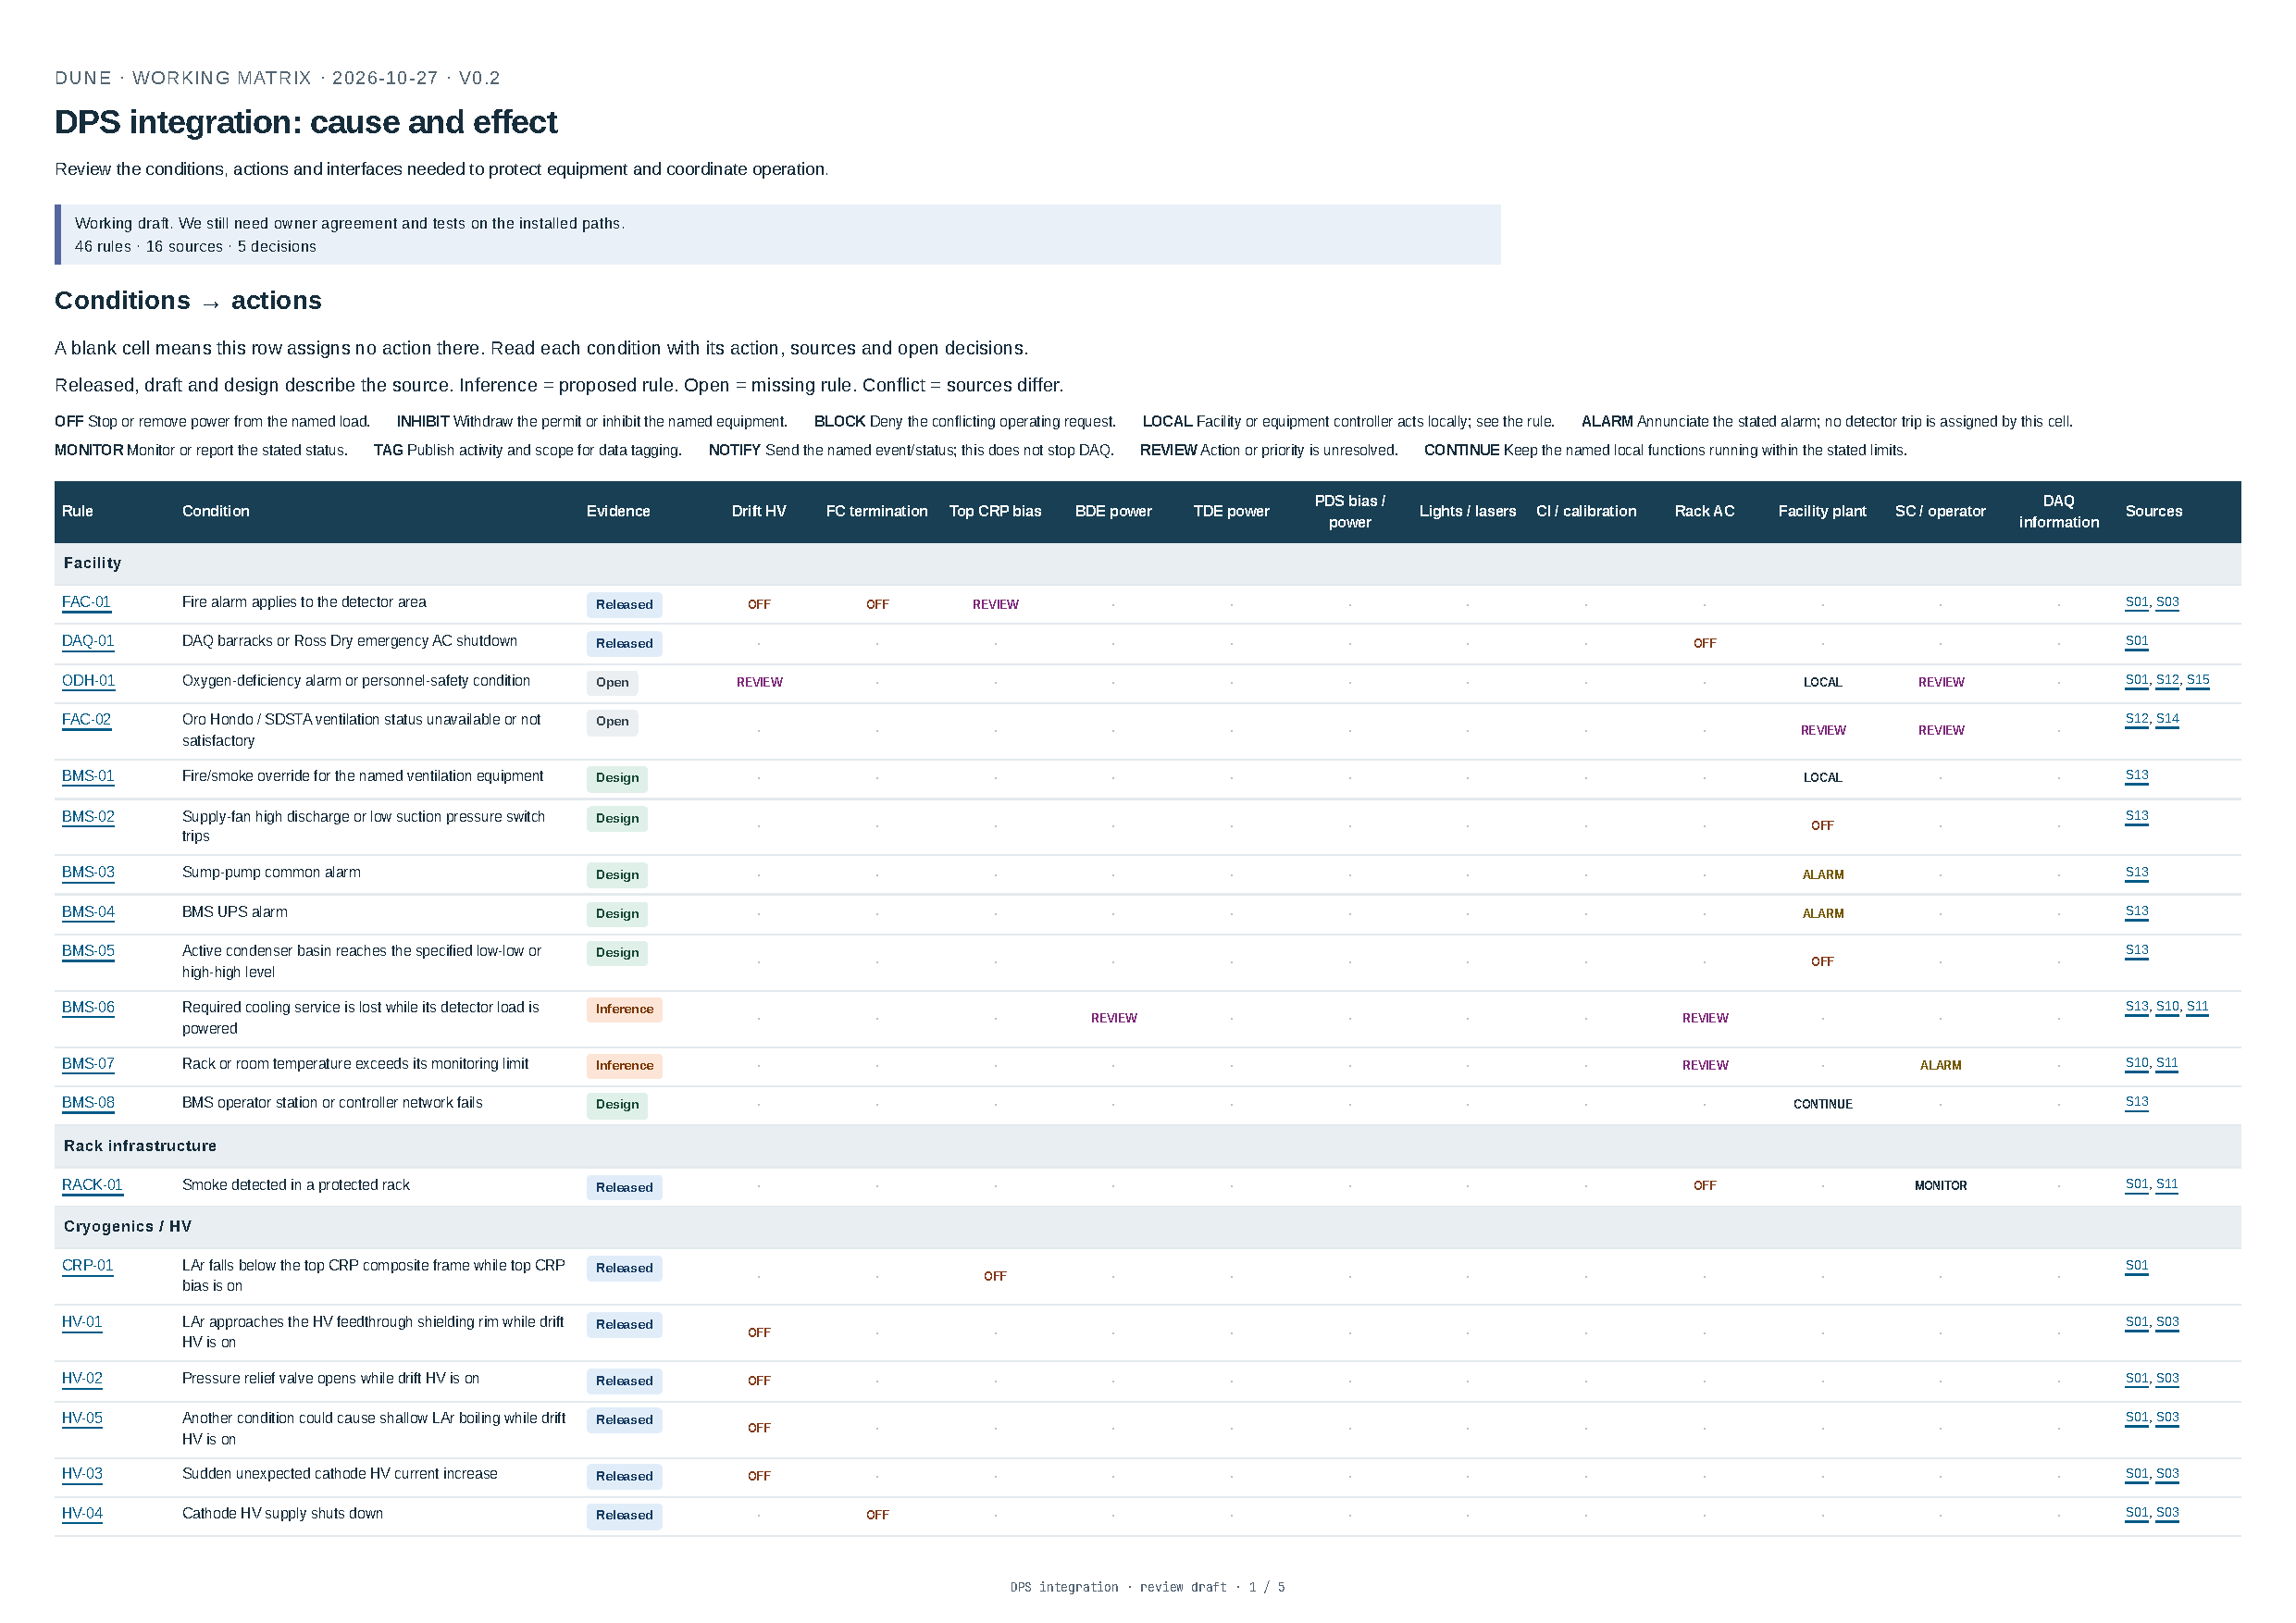
\includegraphics[page=1,width=0.495\linewidth,height=5.8cm,keepaspectratio]{figures/interlock-matrix-v0.2.pdf}\hfill
\includegraphics[page=2,width=0.495\linewidth,height=5.8cm,keepaspectratio]{figures/interlock-matrix-v0.2.pdf}\par\medskip
\raggedright\DuneDiagramCaption{Working matrix v0.2, 27 October 2026, conditions/action pages 1--2. The five-page companion also contains sources, decisions and readiness notes.}
\end{frame}


% Matrix and planning detail moved from the main talk on 12 November 2026.
\begin{frame}{Use the interlock matrix to track each protection function}
\textbf{Working matrix v0.2: 46 rules. Owner agreement and tests remain open.}\par\medskip
% Readable excerpt of the existing integration matrix v0.2 (27 October 2026).
% Exact action cells are retained; condition/evidence labels are abbreviated.
% Complete selected records and input hash: interlock-matrix-excerpt.json.
\begingroup
\small
\renewcommand{\arraystretch}{1.3}
\begin{tabularx}{\textwidth}{@{}>{\RaggedRight\arraybackslash}X*{5}{>{\centering\arraybackslash}p{1.4cm}}>{\RaggedRight\arraybackslash}p{2cm}@{}}
\toprule
\textbf{Condition} & \textbf{HV} & \textbf{BDE} & \textbf{PDS} & \textbf{Rack AC} & \textbf{DAQ} & \textbf{Evidence}\\\midrule
Low LAr level & OFF & -- & -- & -- & -- & Released\\
BDE fan fault & -- & INHIBIT & -- & -- & -- & Inference\\
PDS overcurrent & -- & -- & OFF & -- & -- & Released\\
Rack smoke & -- & -- & -- & OFF & -- & Released\\
PrM lamp active & -- & -- & REVIEW & -- & REVIEW & Conflict\\
LCM calibration & -- & -- & -- & -- & TAG & Draft\\
\bottomrule
\end{tabularx}
\endgroup
\par\medskip
\captionline{Excerpt: a dash assigns no action; REVIEW is unresolved; TAG records activity. Evidence describes the source, not approval or a passed test.}\par\medskip
\textbf{For each function:} source, physical path, action, feedback, timing and reviewer.
\end{frame}

\begin{frame}{Measure milestones with completed records and evidence}
\textbf{Proposed delivery checks}\par\medskip
\renewcommand{\arraystretch}{1.25}
\begin{tabularx}{\textwidth}{@{}>{\RaggedRight\arraybackslash}p{2.8cm}>{\RaggedRight\arraybackslash}p{6.1cm}>{\RaggedRight\arraybackslash}X@{}}
\toprule
\textbf{Delivery} & \textbf{Evidence to deliver} & \textbf{Progress measure}\\\midrule
Connection collection & Confirmed inventory from each group: endpoints, signal, action, feedback, timing, contact and source. & Complete / required connection records, by consortium and LBNF.\\
Concept review & Functions mapped to hardware and logic; I/O gaps, failure/recovery behaviour, decisions and test plan reviewed. & Reviewed, mapped / in-scope functions; open decisions listed.\\
\bottomrule
\end{tabularx}\par\smallskip
\textbf{Hardware evidence is a separate gate:} passed / planned tests; fault-to-final-state time against the agreed budget; loss, reset and recovery.\par\smallskip
Agree scope and reviewers before counting. Targets: inputs by late January; design by mid-April 2027.
\end{frame}

\begin{frame}{Prepare the hardware review}
\renewcommand{\arraystretch}{1.45}
\begin{tabularx}{\textwidth}{@{}>{\RaggedRight\arraybackslash}p{3.4cm}>{\RaggedRight\arraybackslash}X@{}}
\toprule
\textbf{Work before review} & \textbf{Result}\\\midrule
Trace each inhibit & Existing hardware, additions, cable routes and quantities\\
Test representative paths & Measured trip times, recovery and SC logging\\
Prepare purchases & Panel space, power, drawings, parts, licences, costs and spares\\
\bottomrule
\end{tabularx}\par\bigskip
Order after the readiness review; install to match the site schedule.\par\medskip
Agree the facility-interface and full VD response-matrix review schedule with the consortia and LBNF.
\end{frame}

\end{document}
